\documentclass[9pt]{beamer}
%\setbeameroption{show only notes}
\setbeamersize{text margin left=0pt, text margin right=0pt}
\usetheme{Hannover}
\input ./packages.tex
\input ./macros.tex

\title{%
Britain's entrance to China
}

\titlegraphic{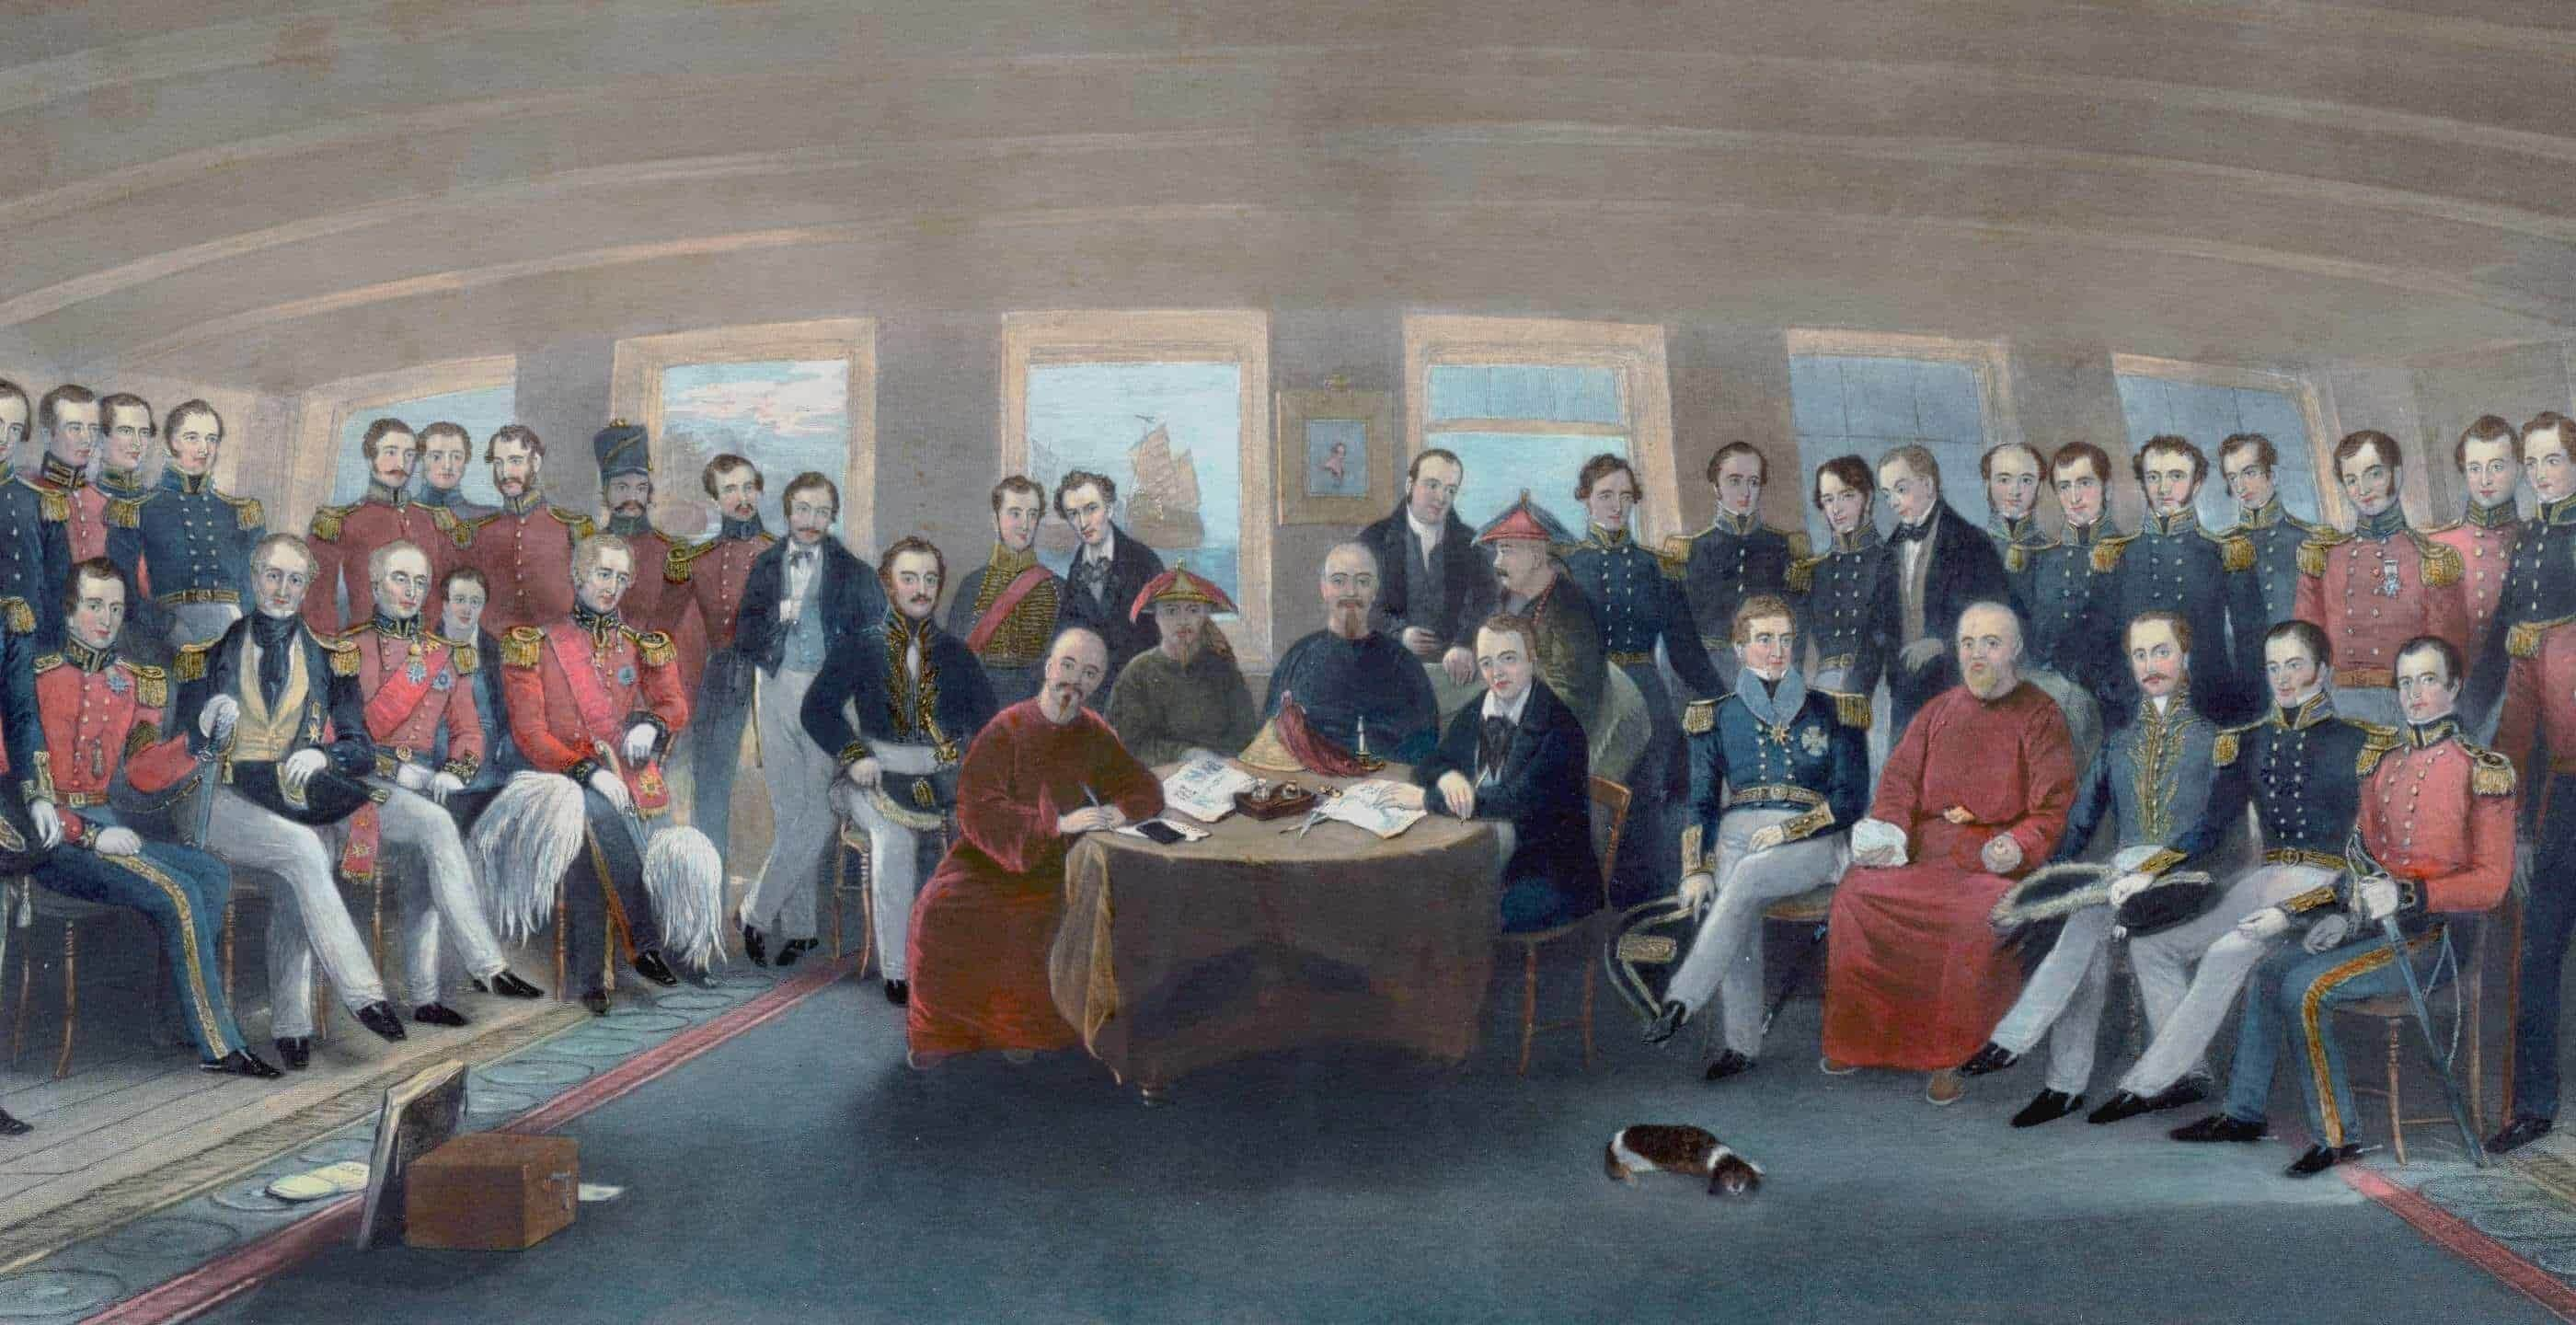
\includegraphics[width=0.8\textwidth]{title}}

\author{Adam Labuš}
\institute{Gamča, Grösslingová 18}

\begin{document}

\begin{frame}
	\pause
	\titlepage
\end{frame}

\begin{frame}
	\frametitle{Structure}
	\tableofcontents
\end{frame}

%Od prveho stretnutia ku vojne
%objavenie caju Wallacom
%prva bojova lod
%klamstva imperatora
%opiody
%zabratie Maoca
%prva vojna

\section{China prologue}

\begin{frame}
	\frametitle{China in the period of European Renaissance, 15th-18th century}
	
	\begin{columns}
		\begin{column}{.5\textwidth}
			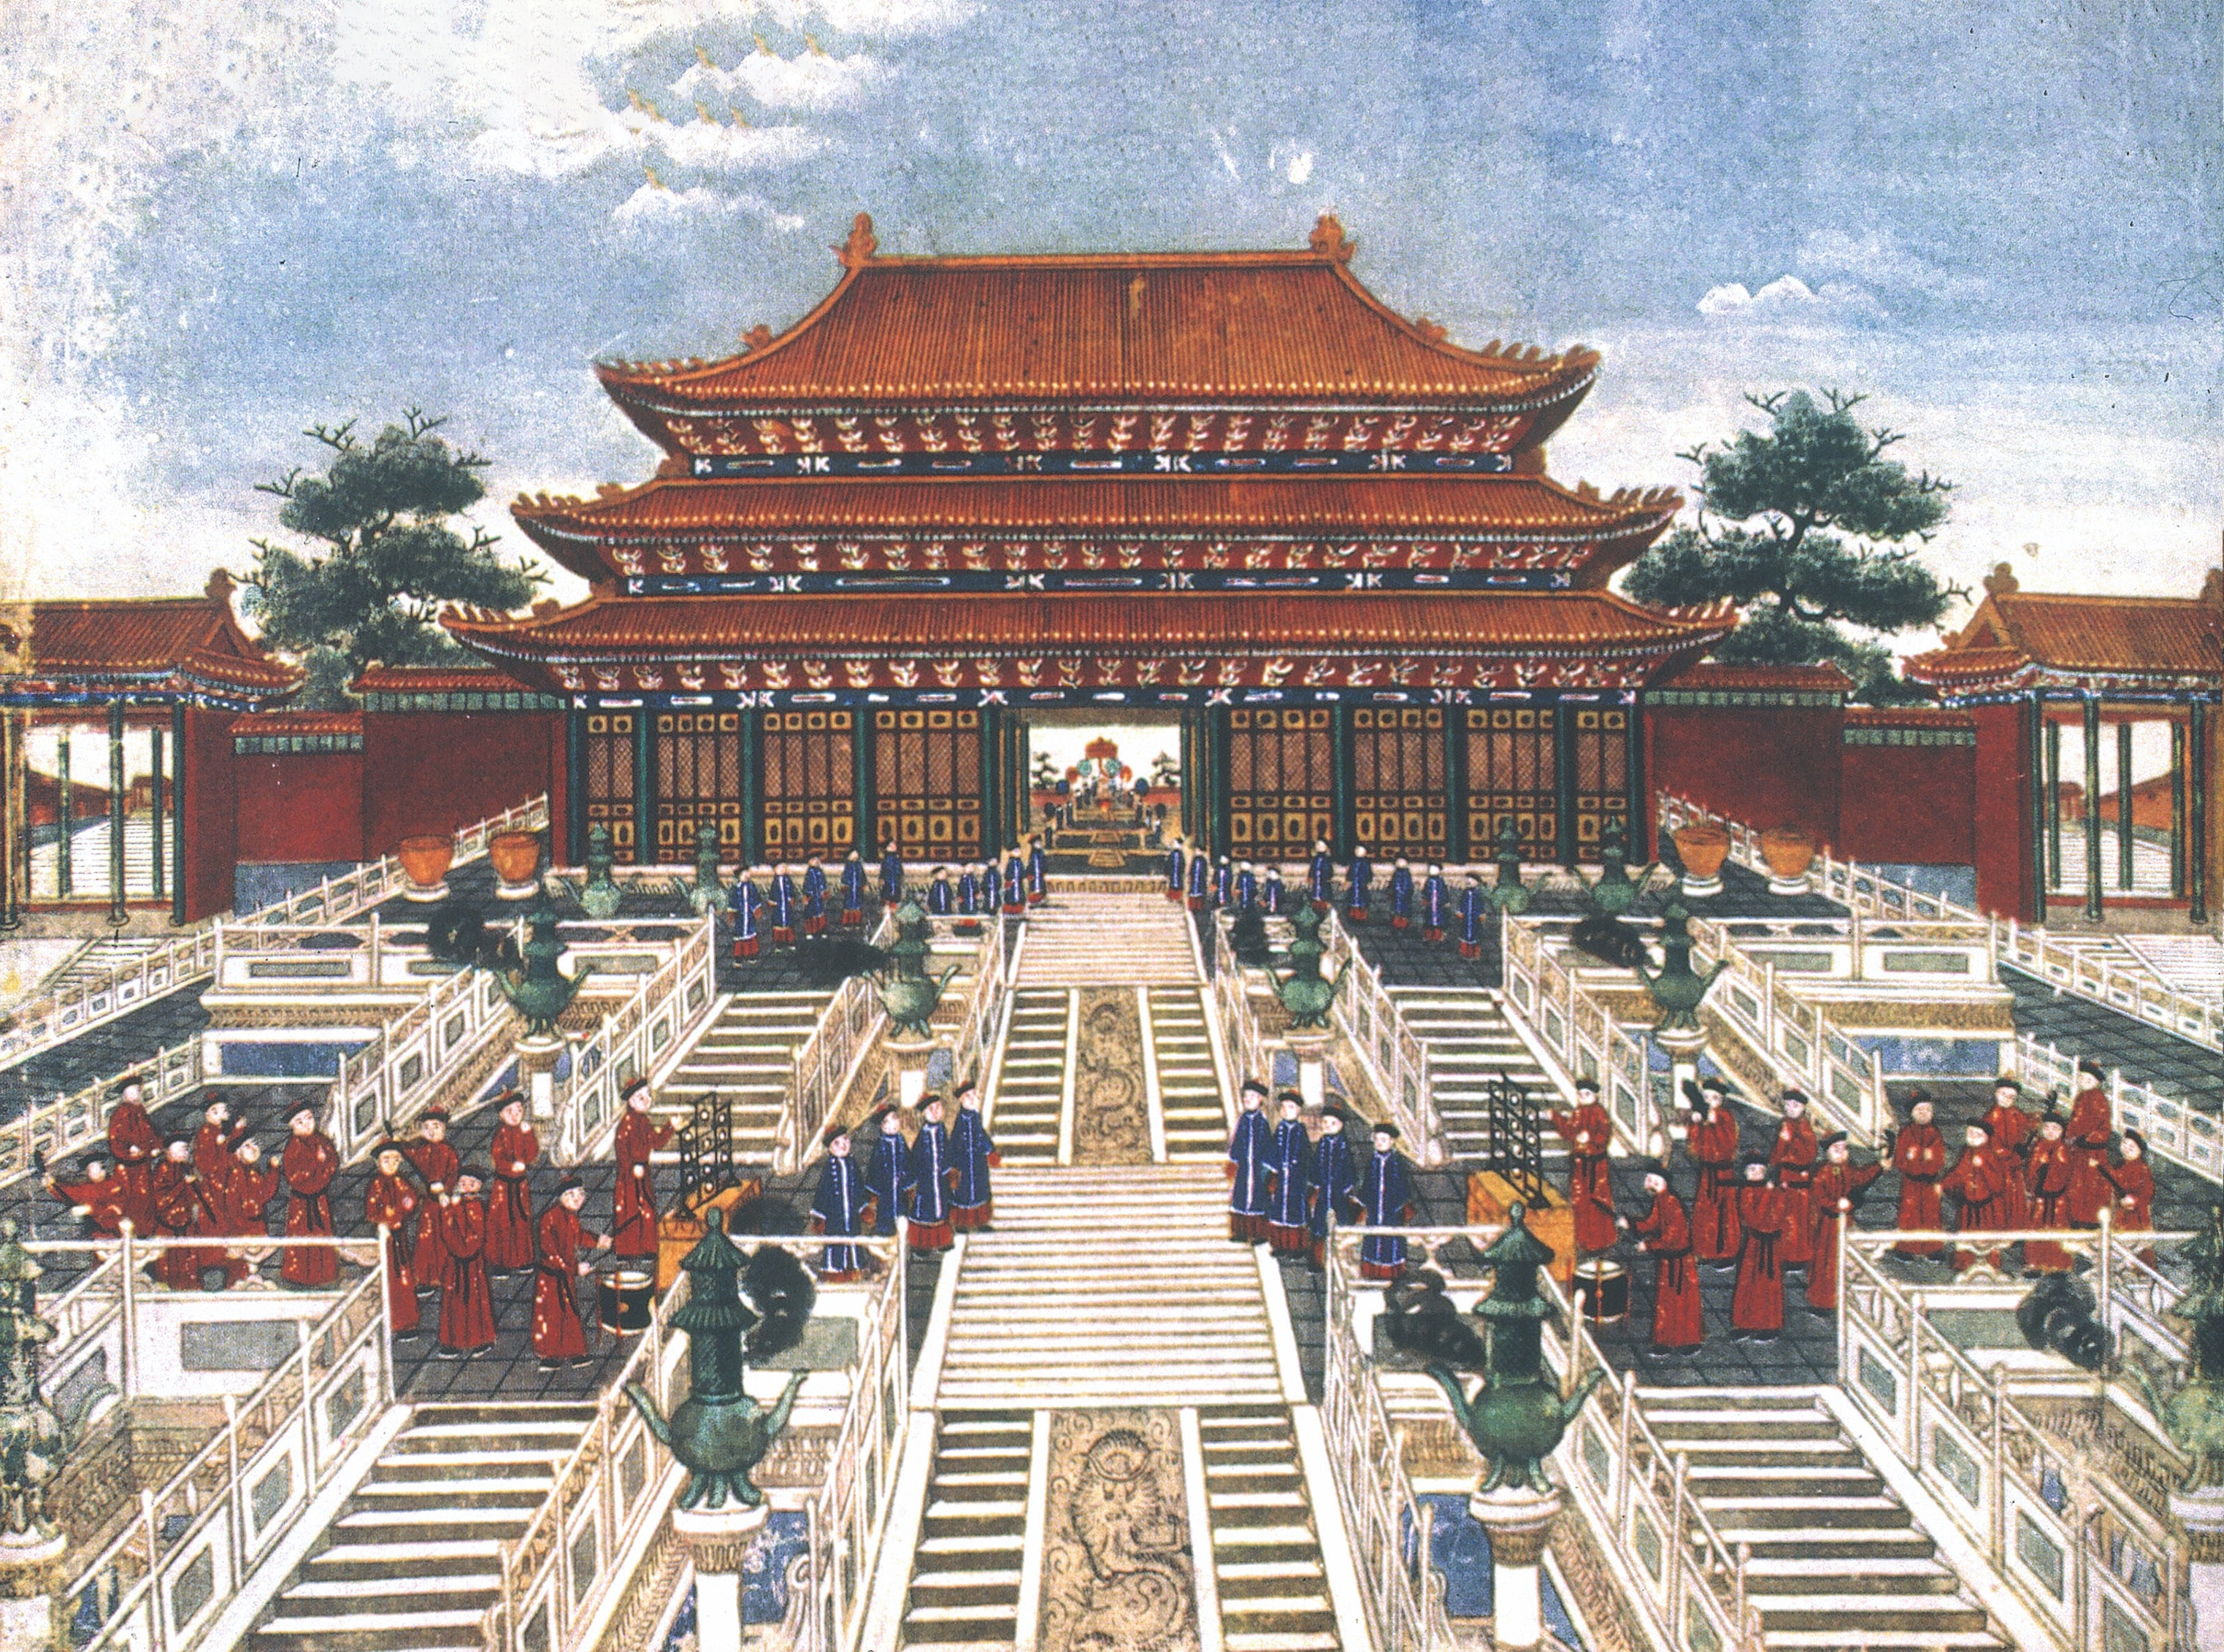
\includegraphics[width=\textwidth]{china-15st}				
		\end{column}
		\begin{column}{.5\textwidth}
			\begin{itemize}
				\item largest country on earth
				\item ruled by the mandarin
				\item cosmological system
			\end{itemize}
		\end{column}
	\end{columns}
	\note{

		no maps of europe - Holand encounter
		cosmological system:
			- Bejing center of the universe between Heaven and Earth
			- emperor is the Son of God
			- all around china were tribal lands
	}
\end{frame}

\begin{frame}
	\frametitle{Canton}

	\begin{columns}
		\begin{column}{.5\textwidth}
			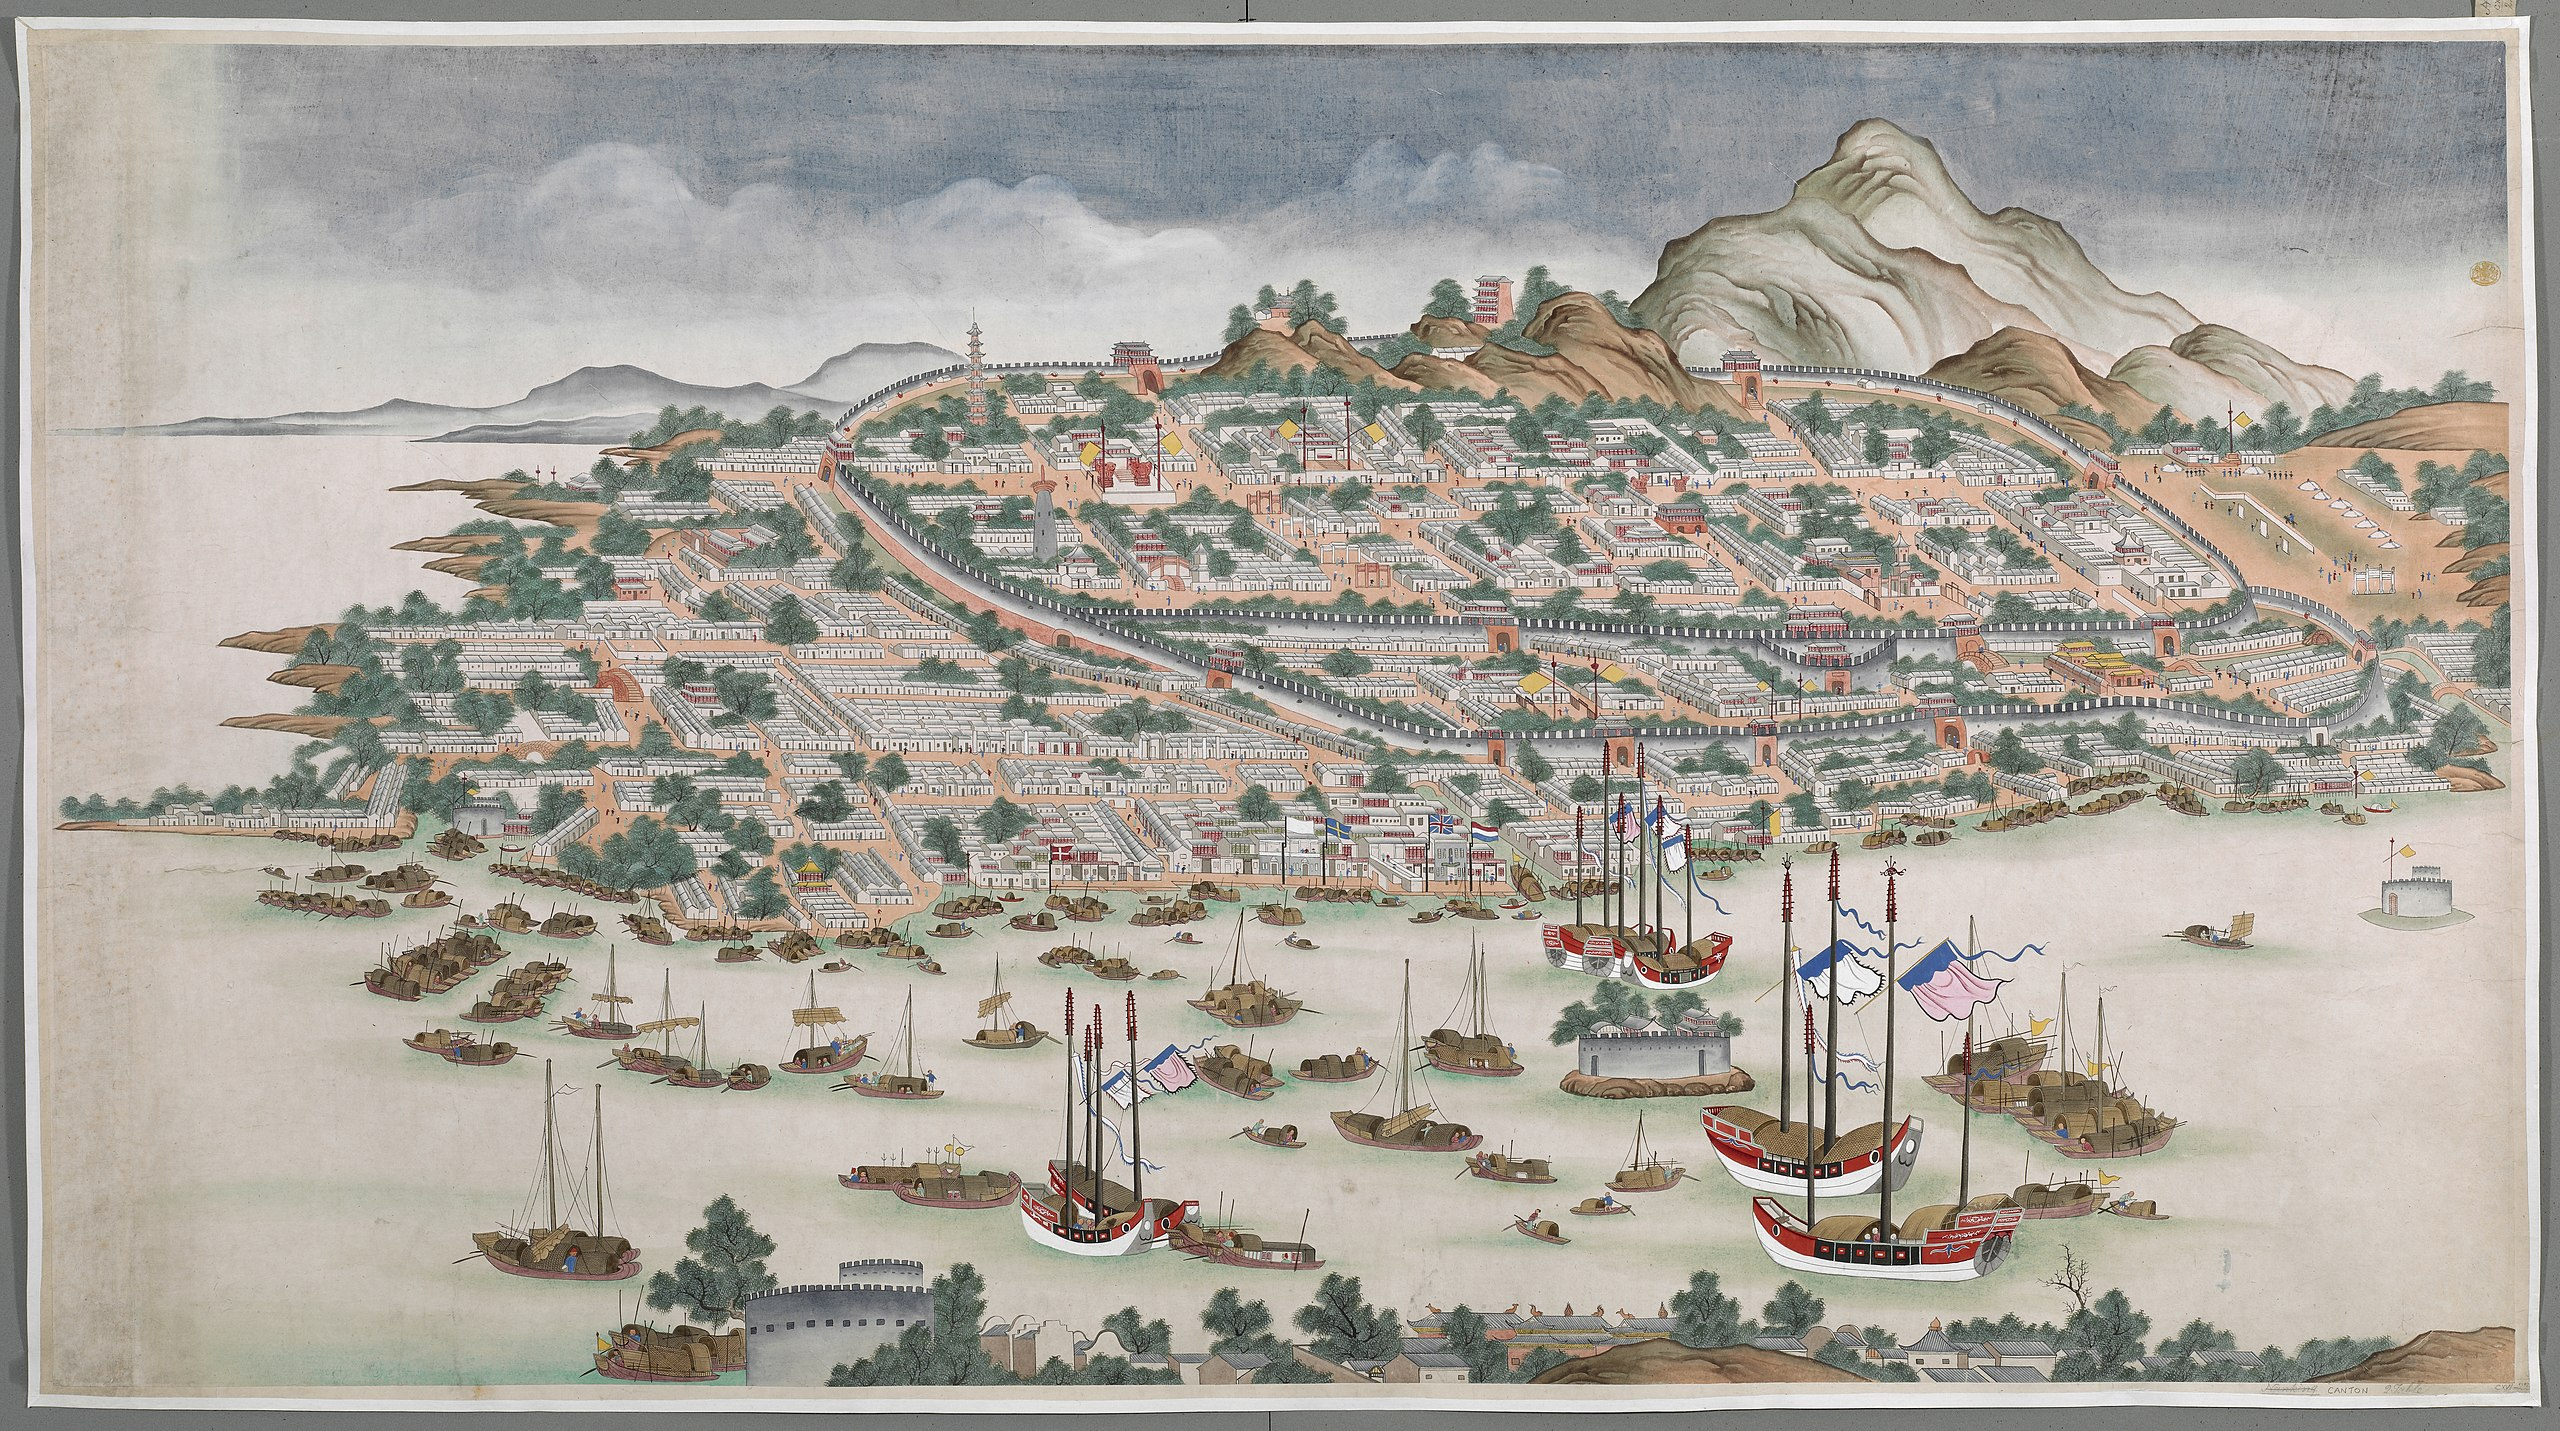
\includegraphics[width=\textwidth]{canton}
		\end{column}
		\begin{column}{.5\textwidth}
			\begin{itemize}
				\item capital of the chineese south
				\item much larger than cities in Europe
			\end{itemize}
		\end{column}
	\end{columns}

	\note{
		focused in the north
	}
\end{frame}

\begin{frame}
	\frametitle{Mocau}

	\begin{columns}
		\begin{column}{.5\textwidth}
			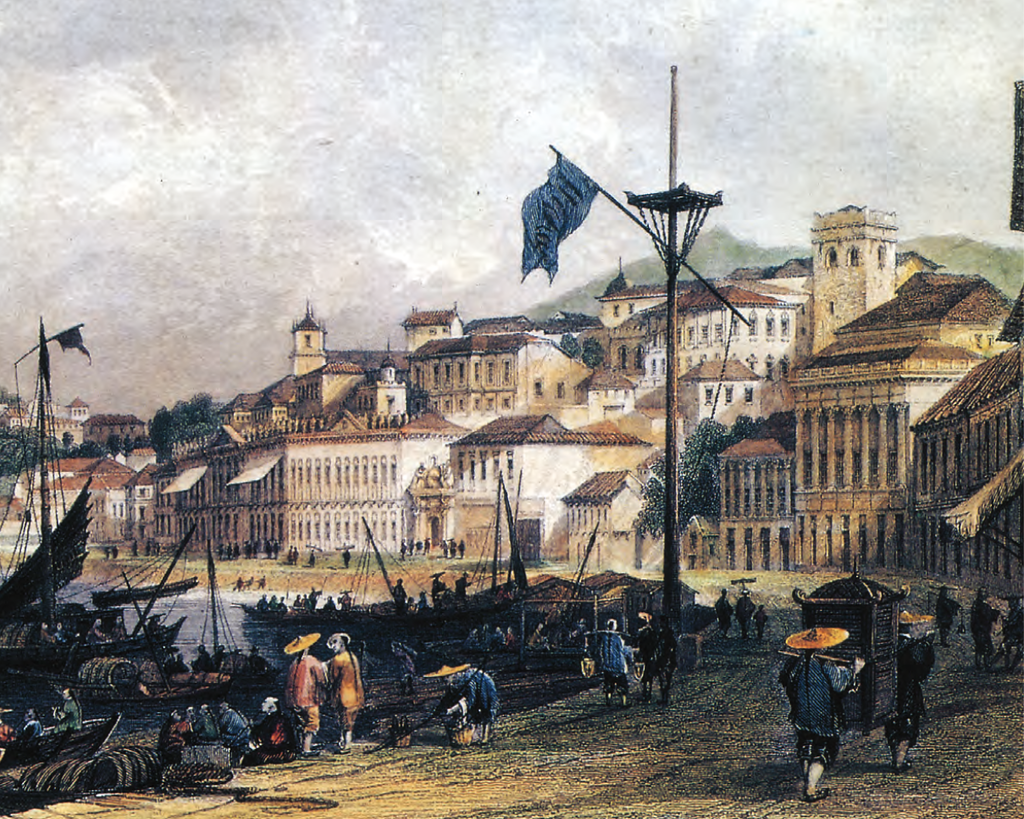
\includegraphics[width=\textwidth]{mocau}
		\end{column}
		\begin{column}{.5\textwidth}
			\begin{itemize}
				\item Founded in 1557
				\item Portugeese colony	
			\end{itemize}
		\end{column}
	\end{columns}

	\note{
	}
\end{frame}

\begin{frame}
	\frametitle{Map of Pearl River Delta}
	\centering
	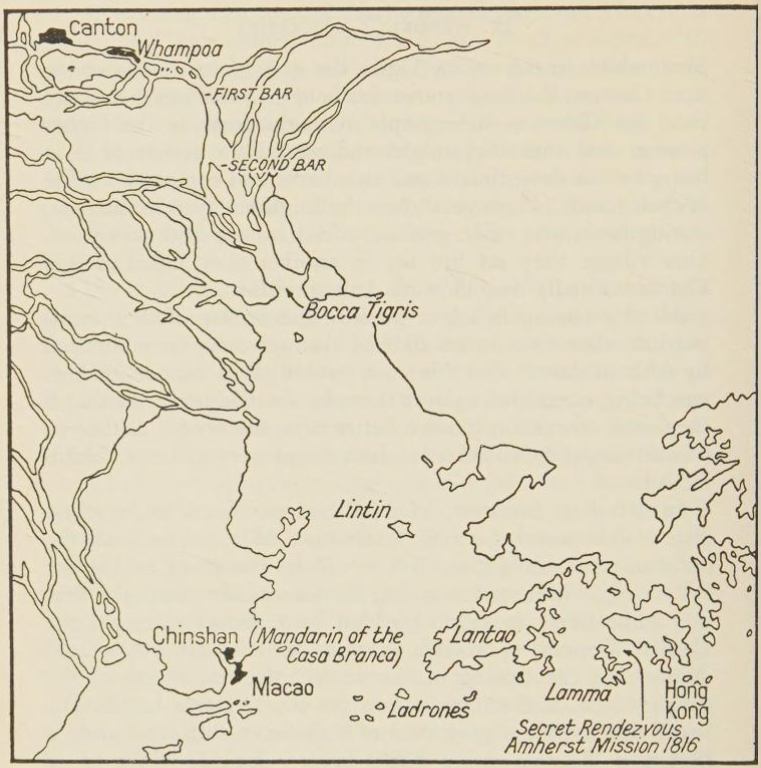
\includegraphics[height=.8\textheight]{map1}

	\note{
		future battlefield
	}
\end{frame}

\section{Encounter with the British}

\begin{frame}
	\frametitle{John Weddel's Voyage to China}
	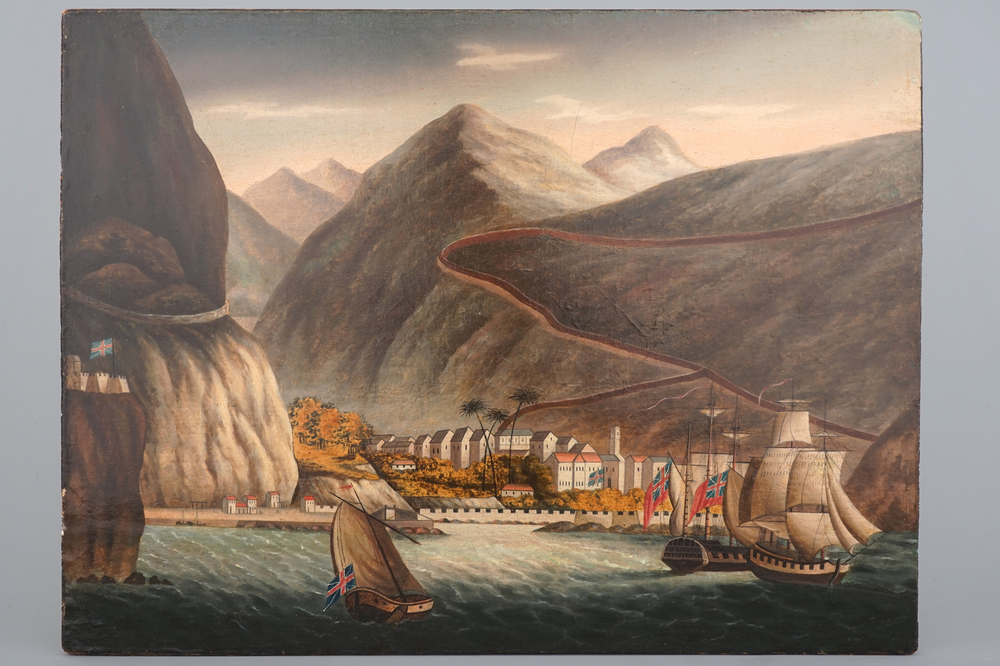
\includegraphics[width=.9\textwidth]{boat}
	\note{
		think that Portugeese are full of shit
	}
\end{frame}

\begin{frame}
	\frametitle{Peter Mundy's diary}
	\LARGE
	\centering
	\vspace{1em}
	\textit{''The people there gave us a certaine Drinke called Chaa,
	which is only water with a kind of herbe boyled in itt. It must bee Drancke warme and is accompted wholesome''}

	\pause
	\vspace{0.5em}
	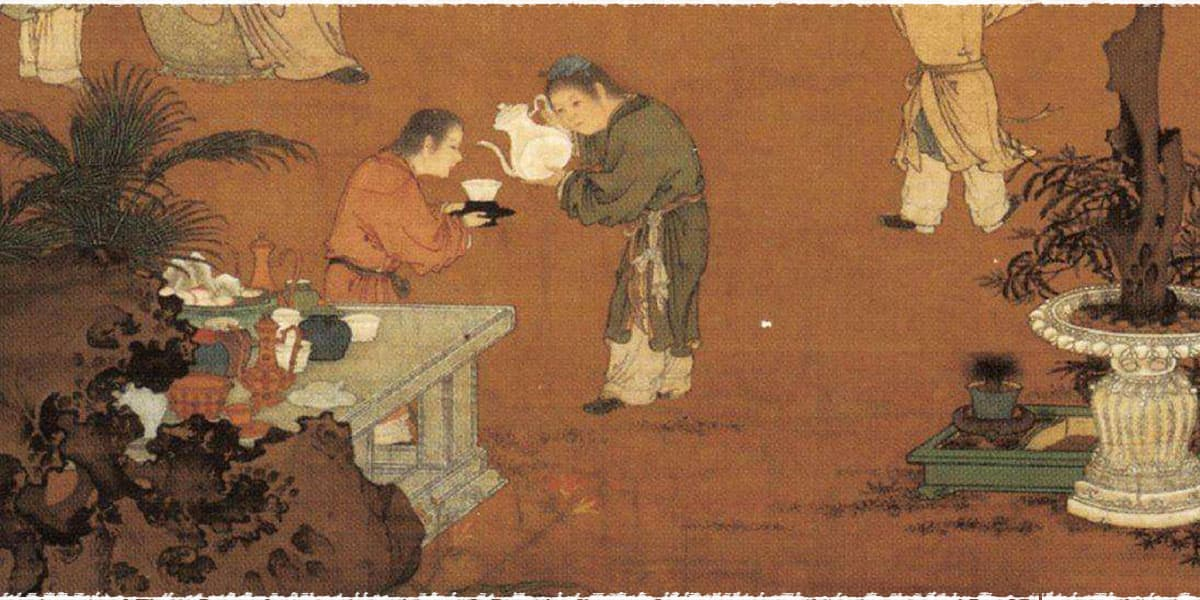
\includegraphics[width=.9\textwidth]{tee}

	\note {
		commercial officer
		wait for permission
		Wddel proceeds, fort open fires
		was china militarily weak or strong
		boats with bombs
		traders were taken hostage in Canton
	}
\end{frame}

\begin{frame}
	\frametitle{Anunghoi Fort}

	\centering
	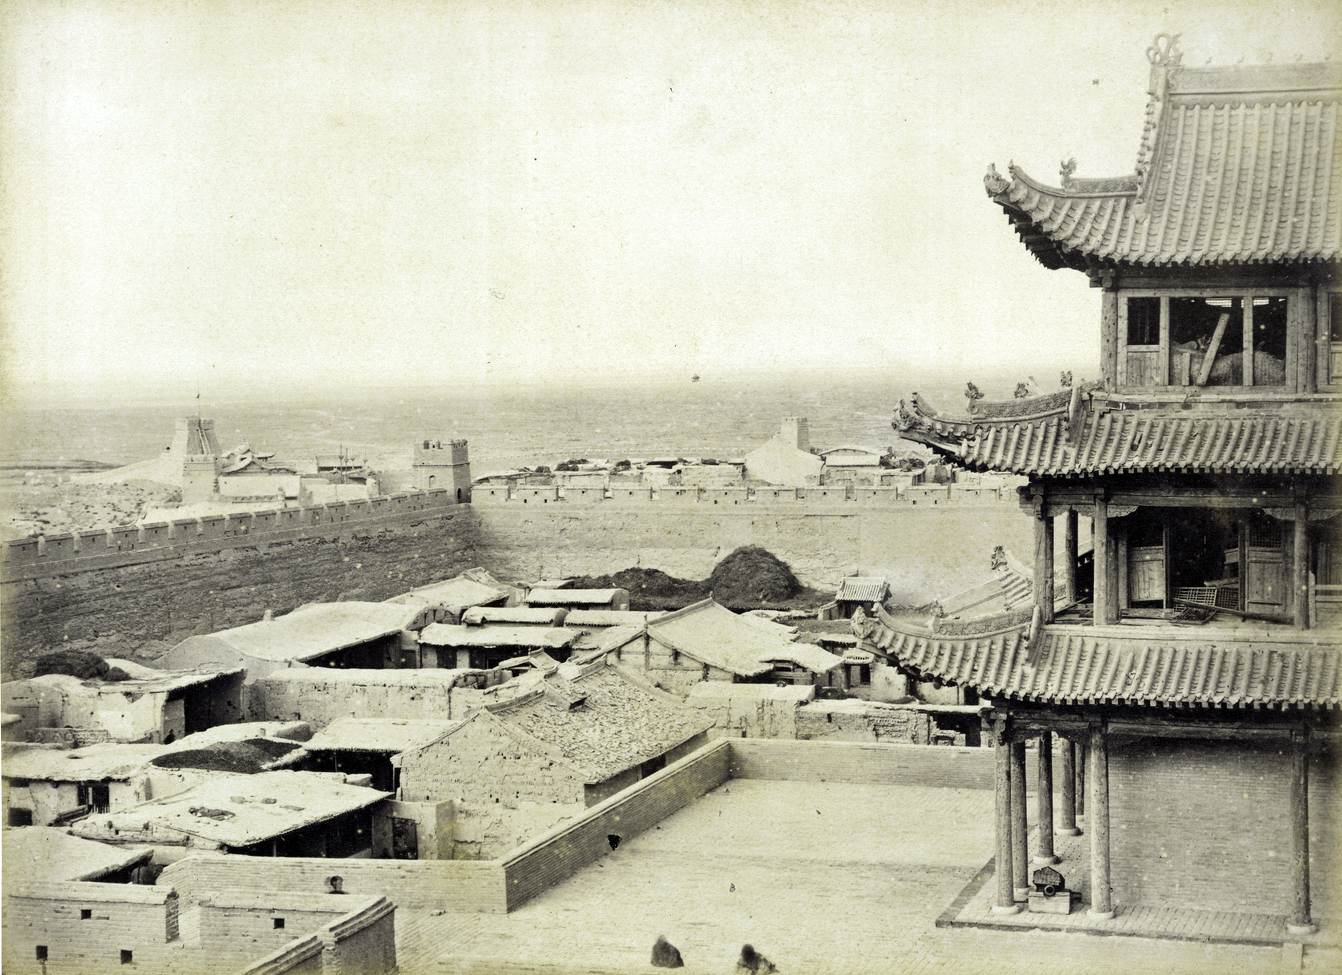
\includegraphics[width=.9\textwidth]{fort}

	\note{
		red haired English with beards, penetrating blue eyes represented the Dutch - red barbarians
	}
\end{frame}


\section{Trade
}
\begin{frame}
	\frametitle{Co-Hong}
	\only<1>{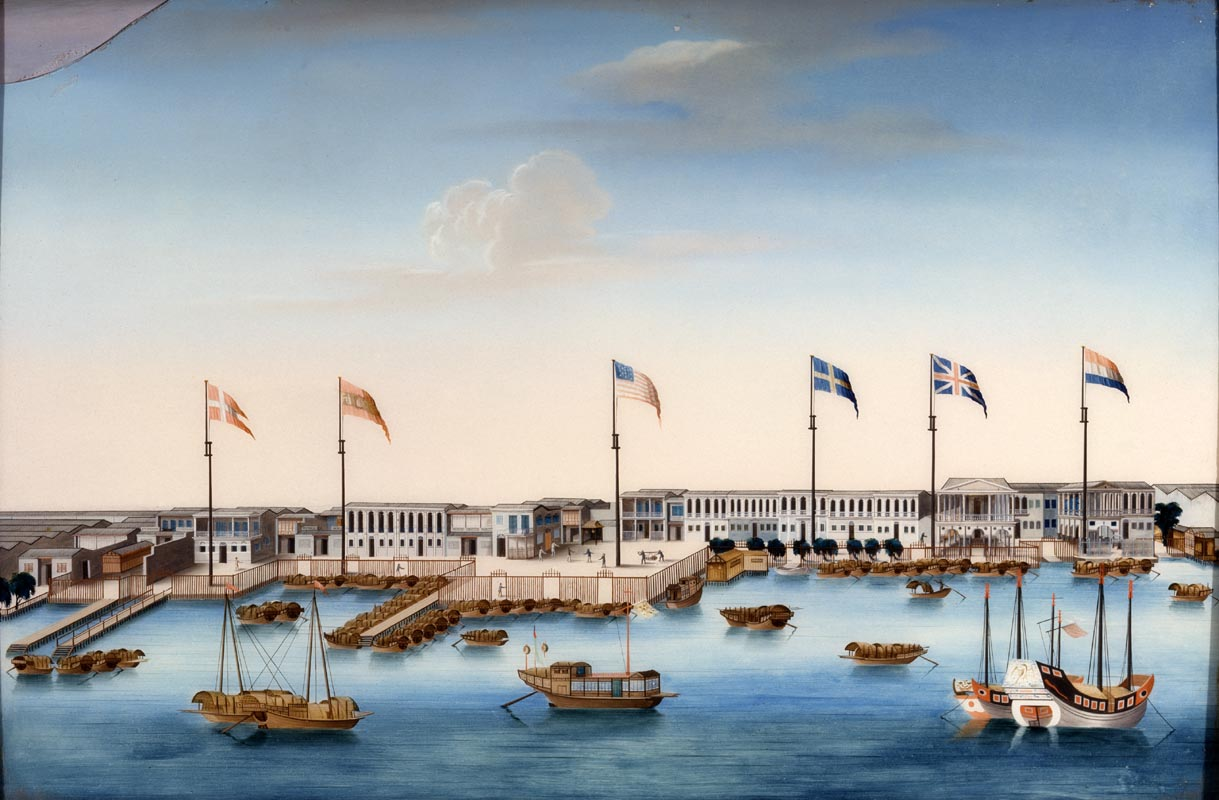
\includegraphics[width=.9\textwidth]{canton_factories}}
	\only<2>{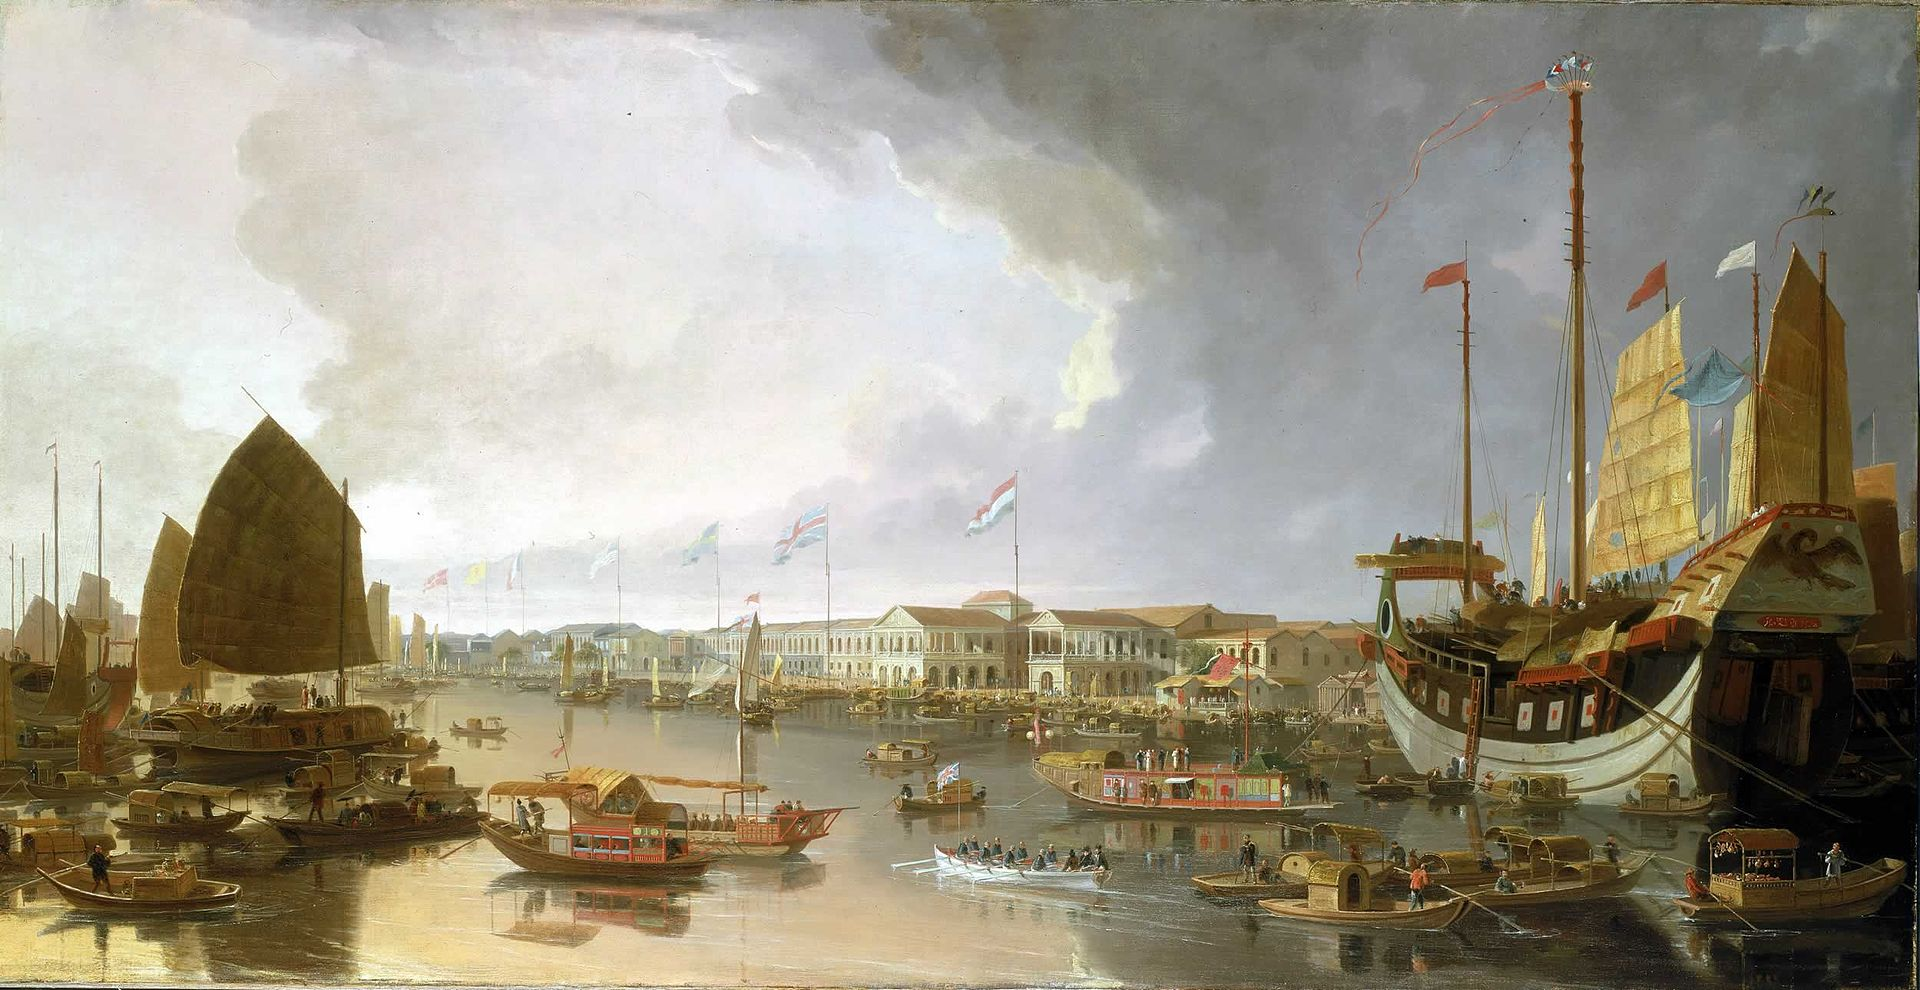
\includegraphics[width=.9\textwidth]{canton_factories2}}
	
	\note{
		The leader was the Hoppo
		the emperor accepted it for profit
	}
\end{frame}

\begin{frame}
	\frametitle{Opium}
	
	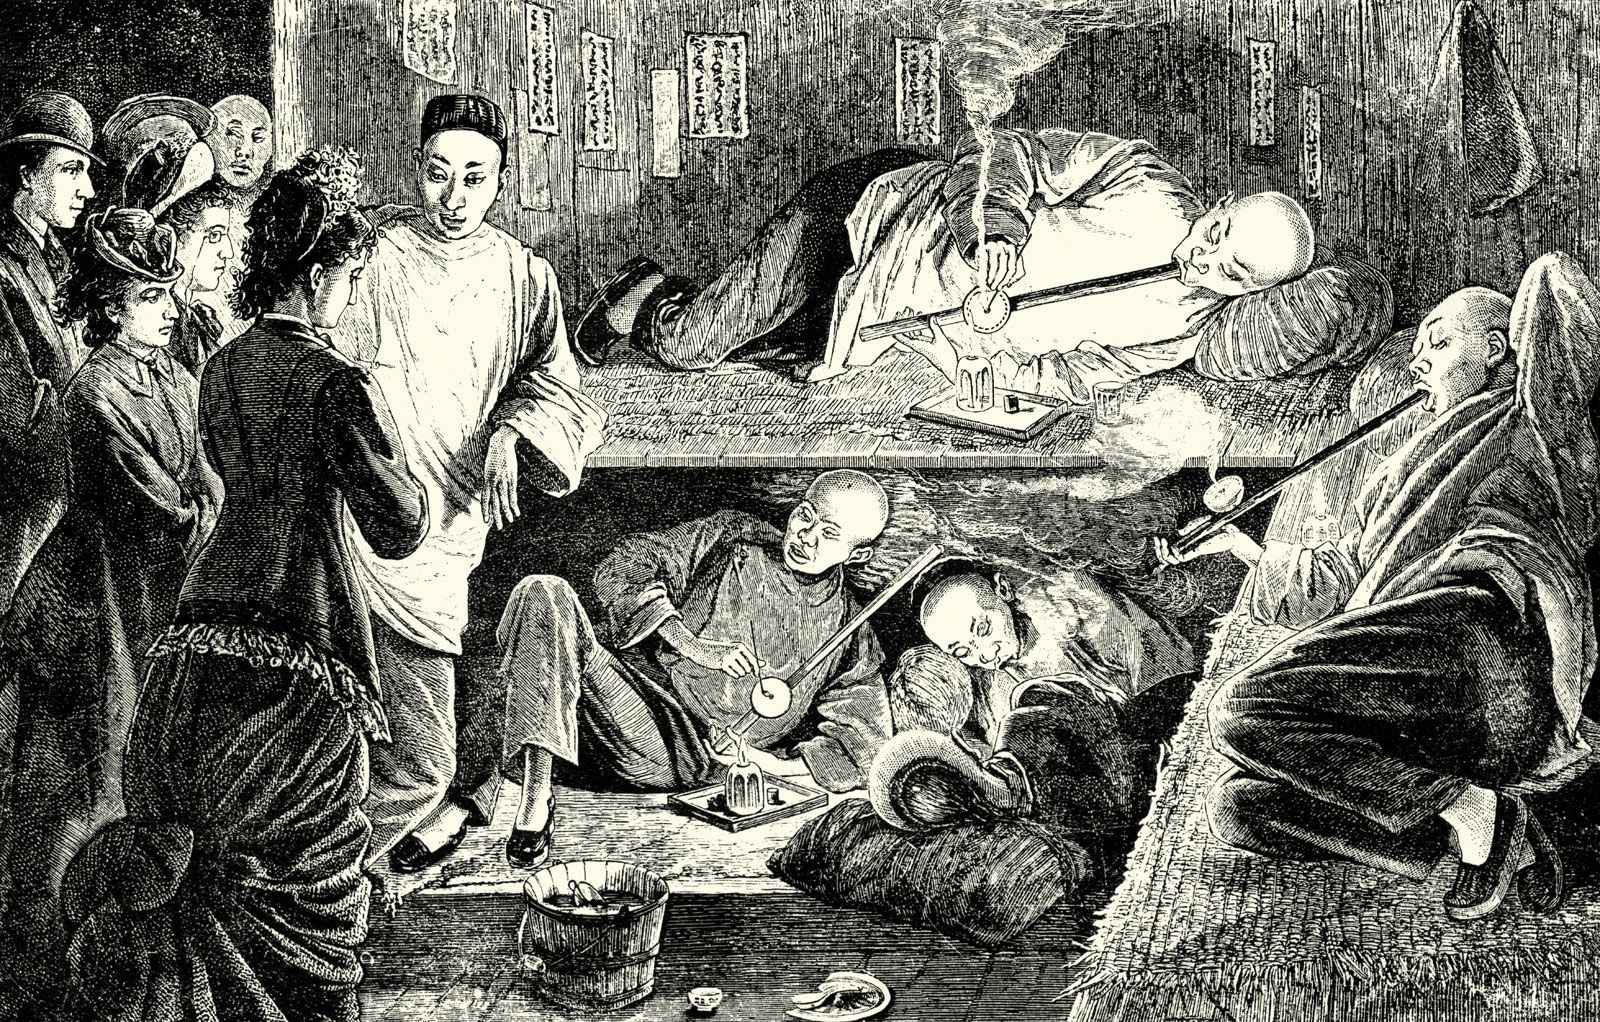
\includegraphics[width=.9\textwidth]{opium}

	\note {
		the east indian company banned it
	}
\end{frame}

\section{Escalation of tensions}

\begin{frame}
	\frametitle{Changing tides - HMS Centurion}

	\begin{columns}
	\begin{column}{.5\textwidth}
	\begin{itemize}
		\item captain John Durell
		\item entered china in 1741
	\end{itemize}
	\end{column}
	\begin{column}{.5\textwidth}
	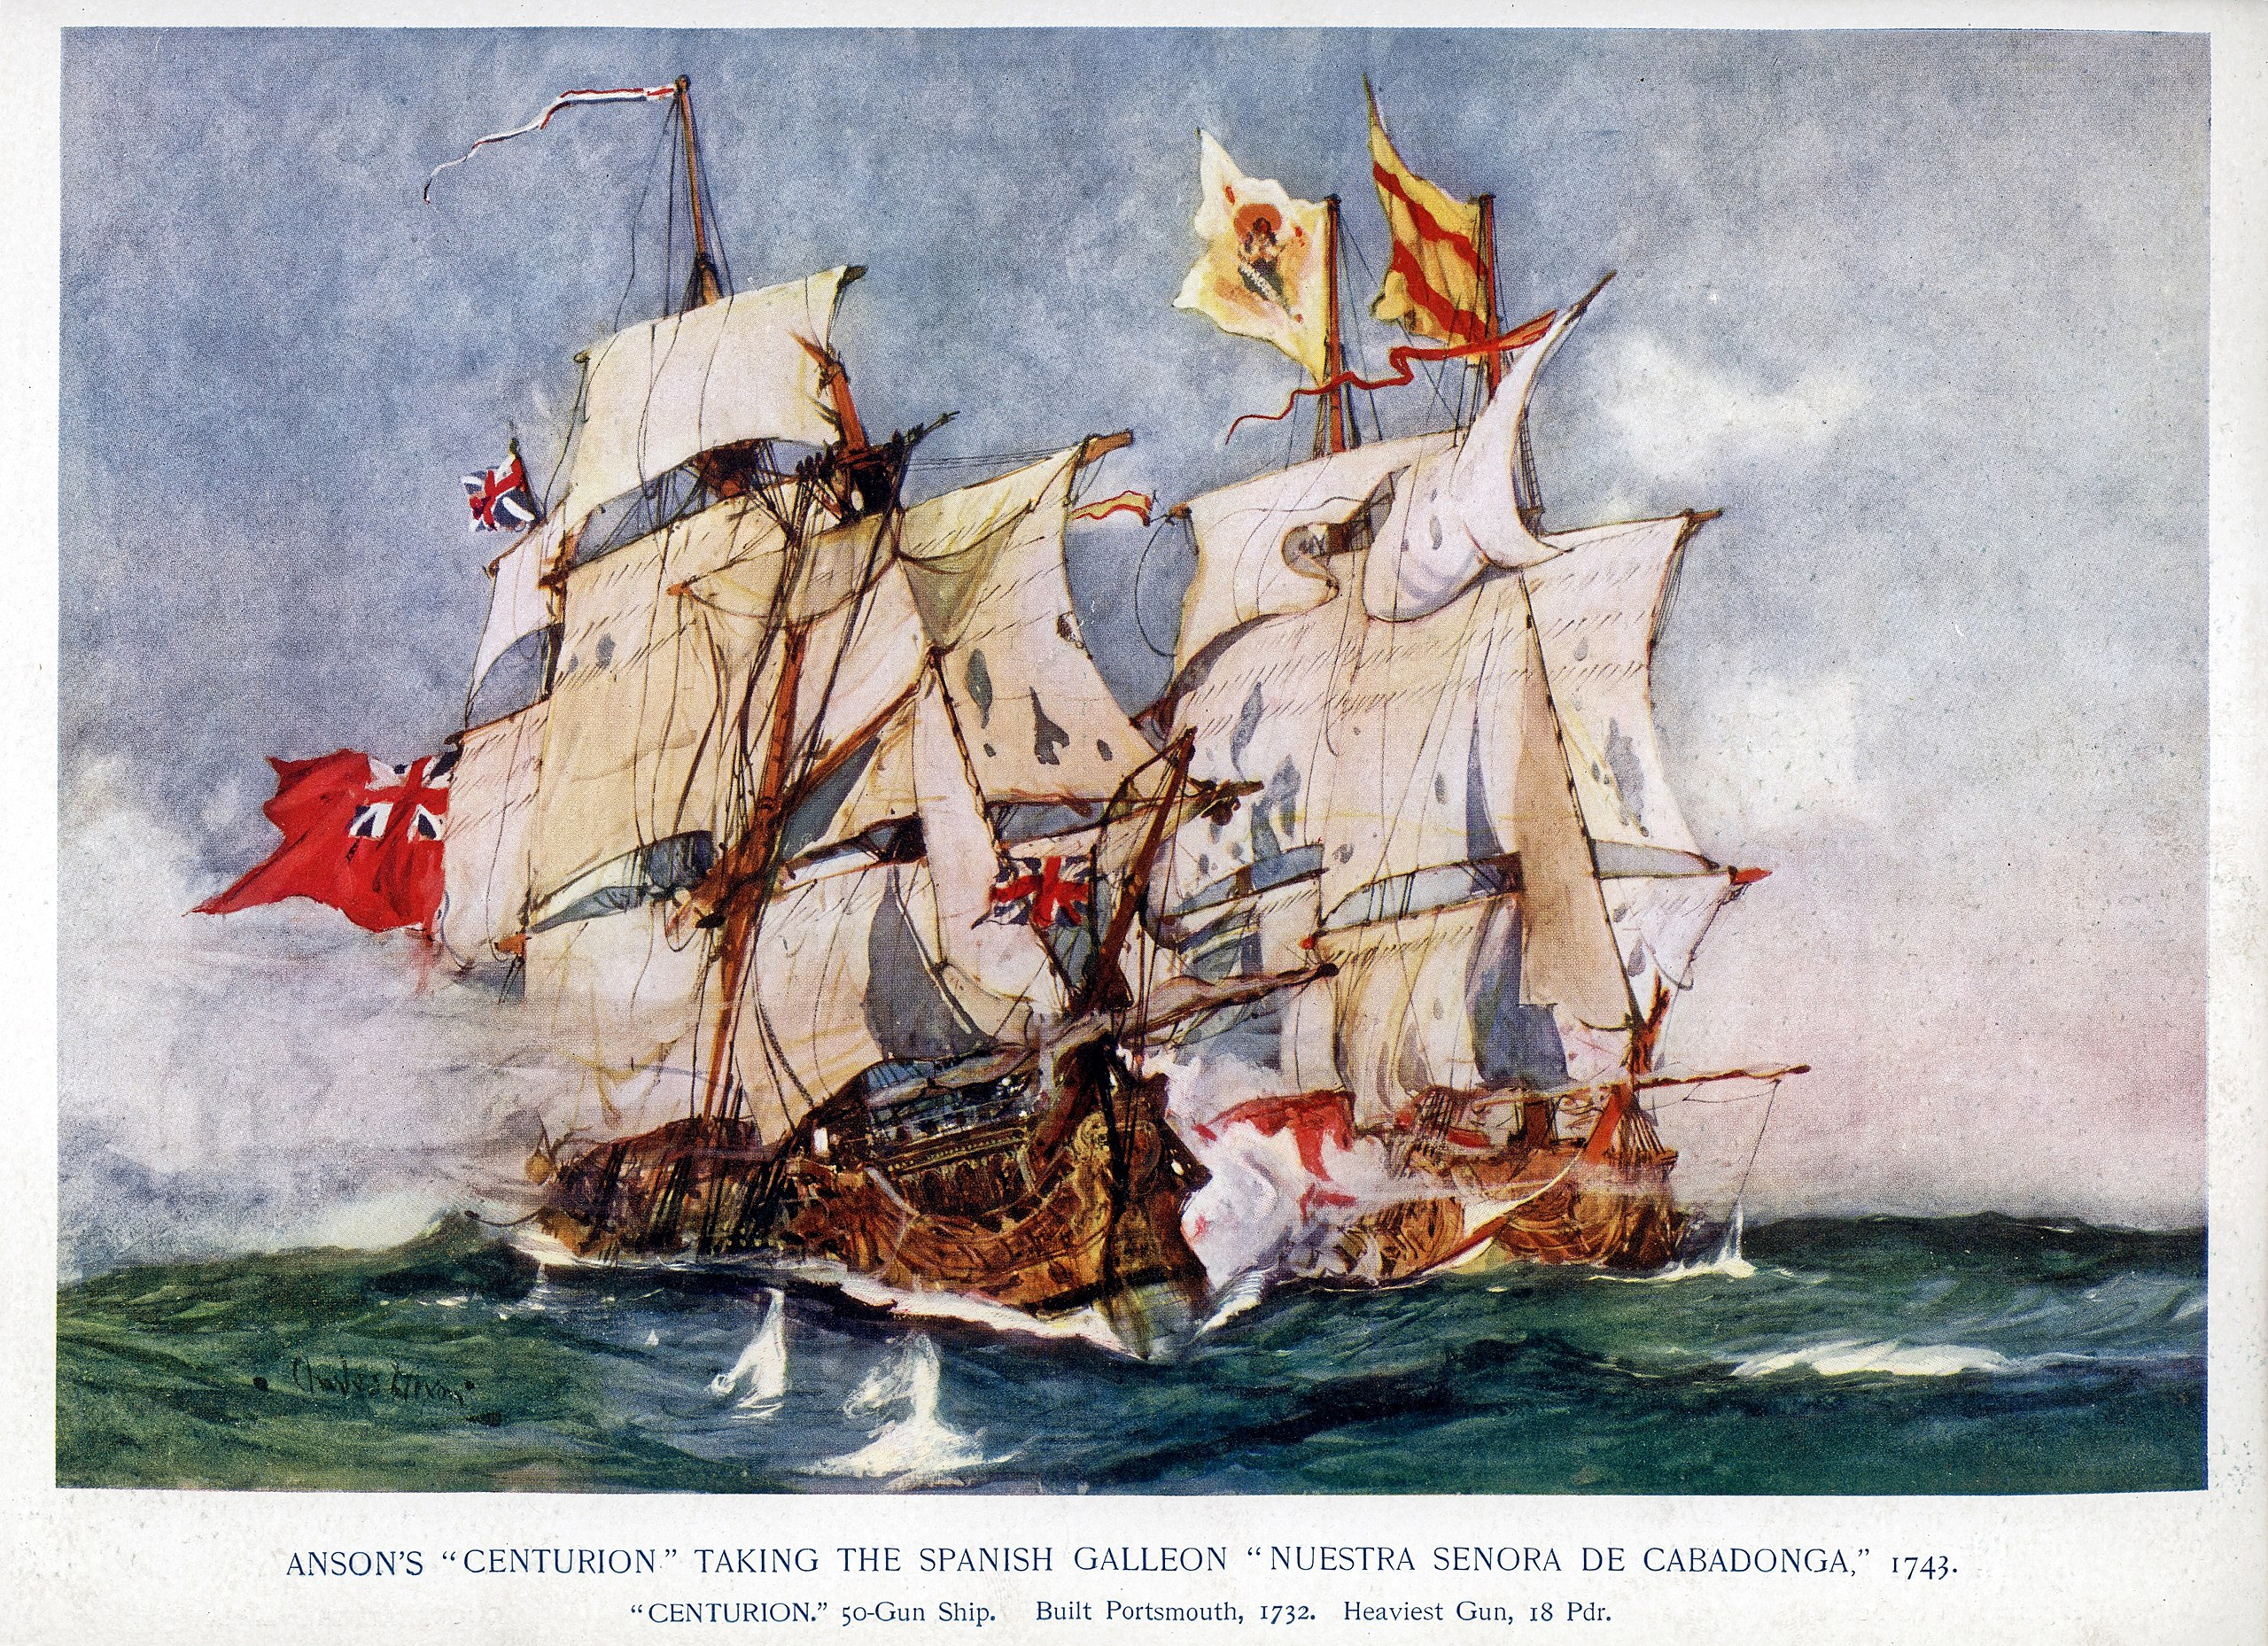
\includegraphics[width=.9\textwidth]{battle_ships}
	\end{column}
	\end{columns}


	\note {
		cleared fire in canton	
	}
\end{frame}

\begin{frame}
	\frametitle{Misifiring of a salute}

	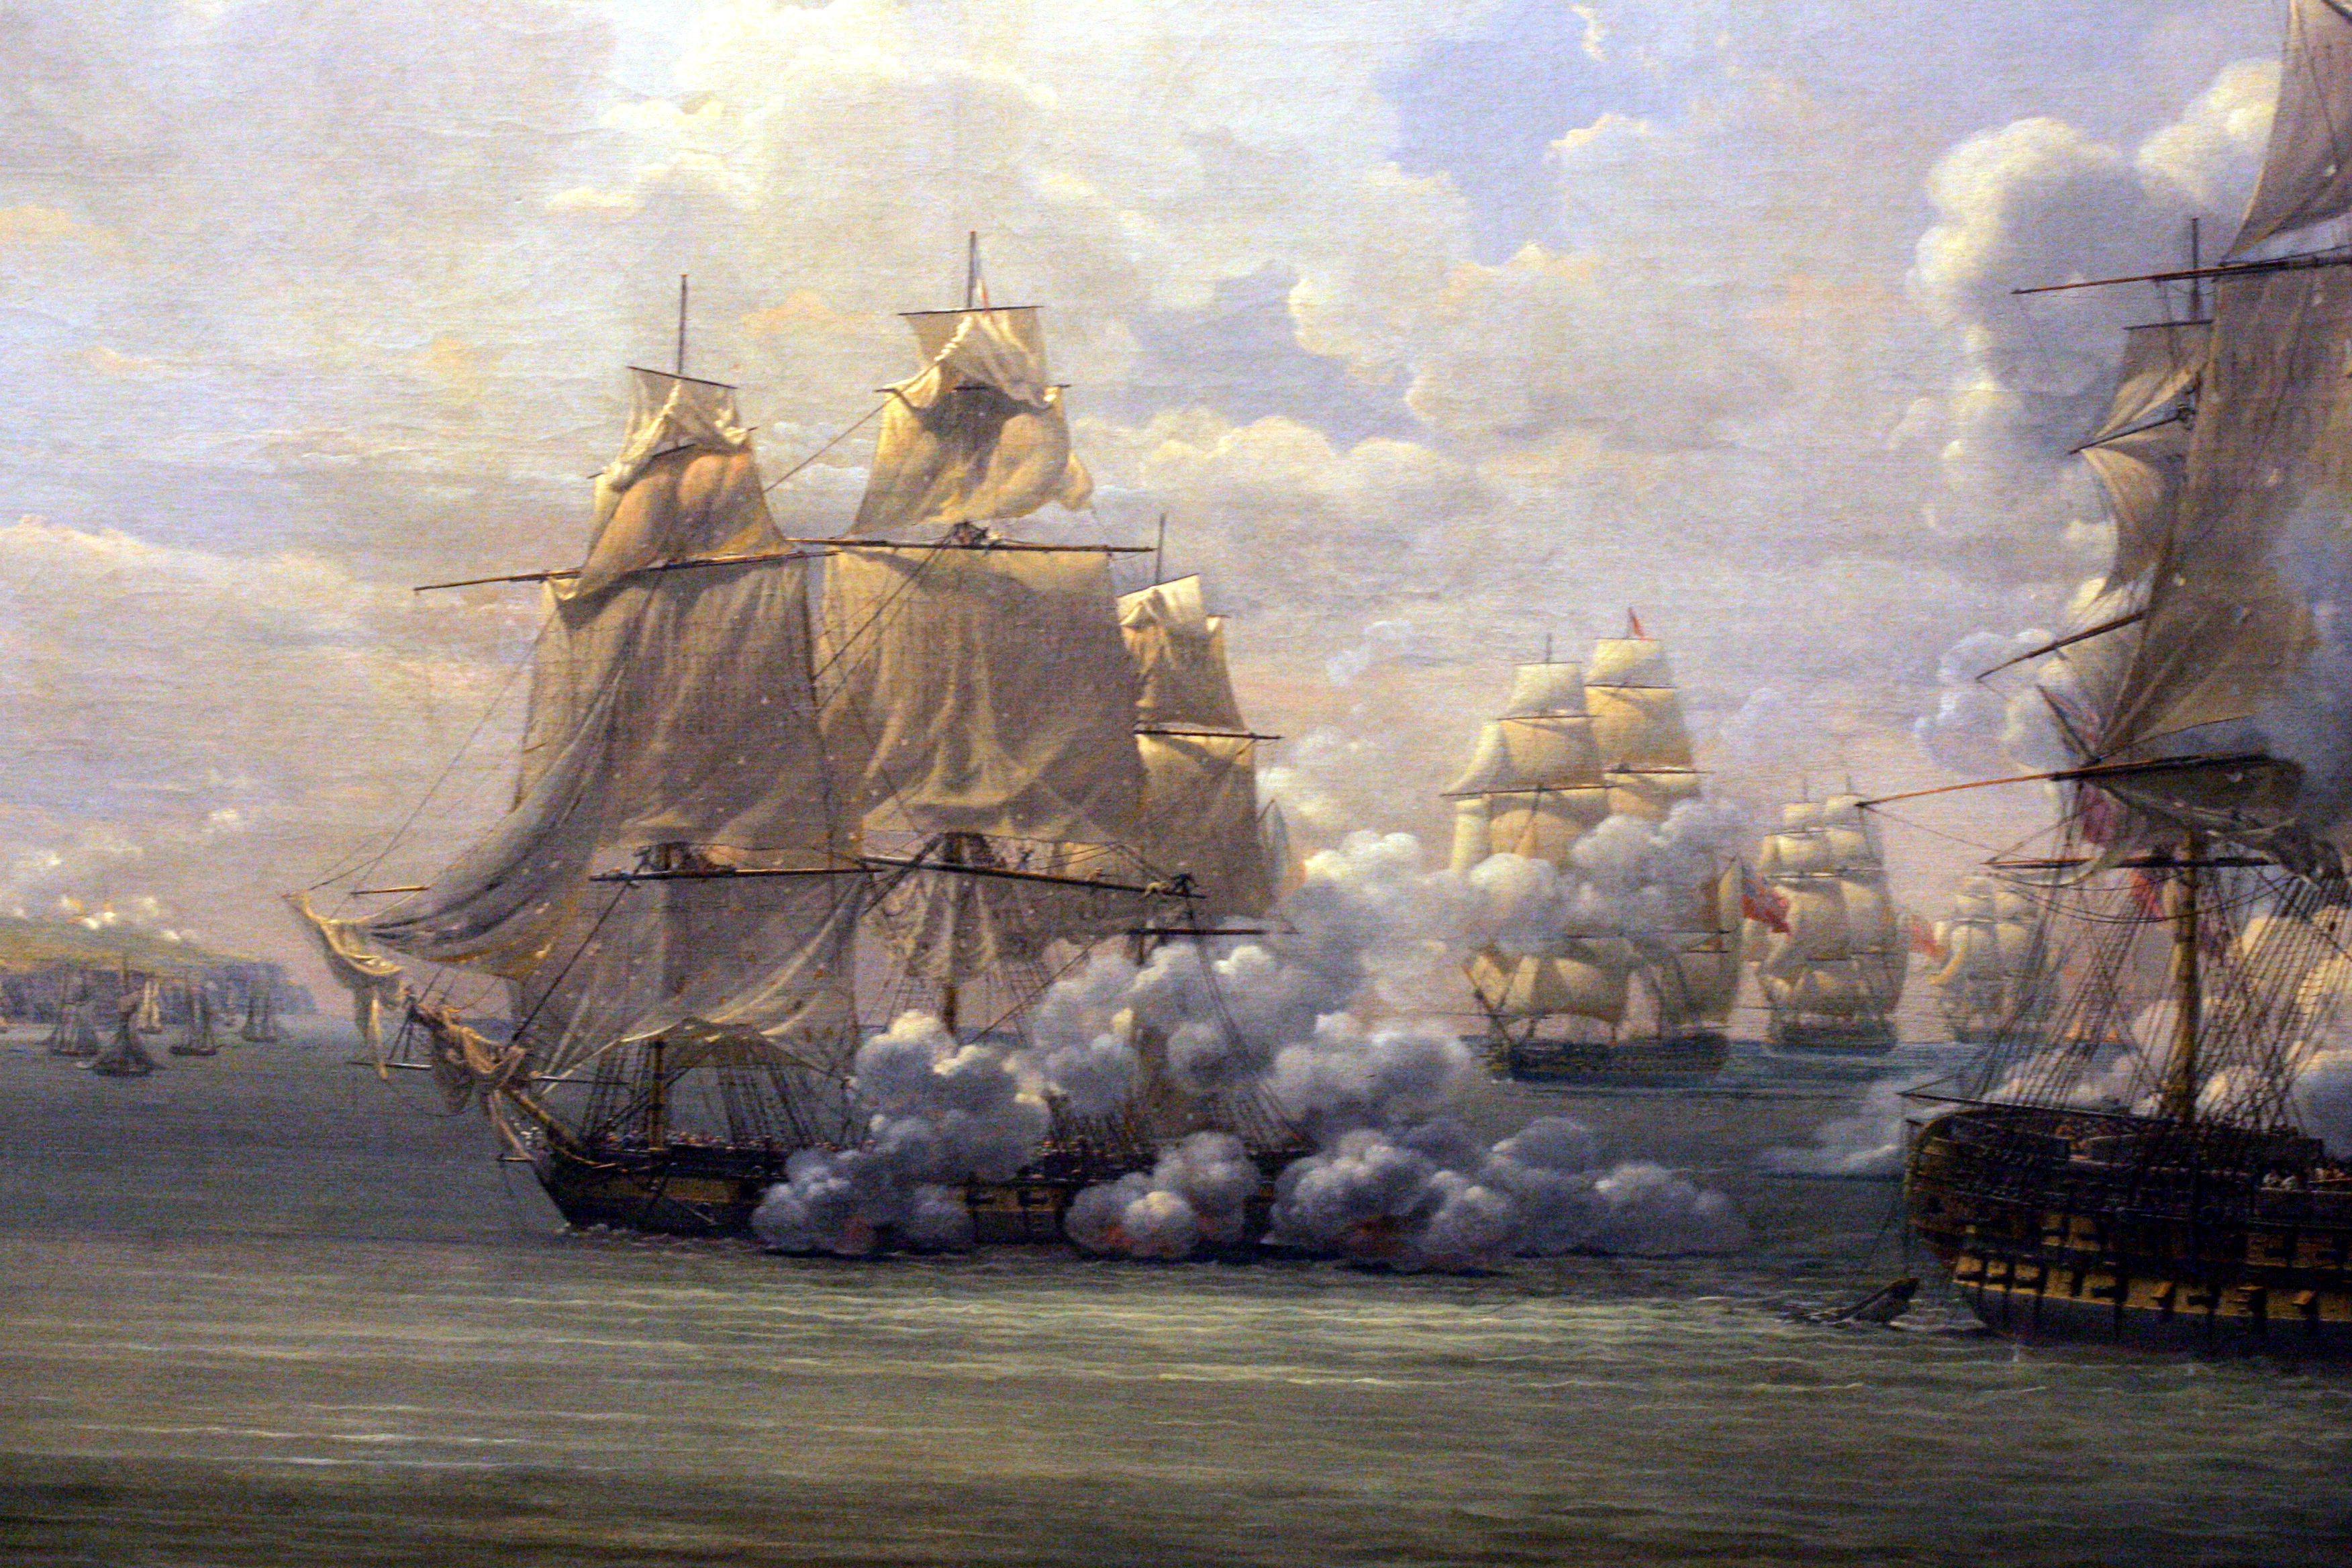
\includegraphics[width=.9\textwidth]{firing}
\end{frame}

\begin{frame}
	\frametitle{British occupation of Mocau and Admiral Drury}

	\centering
	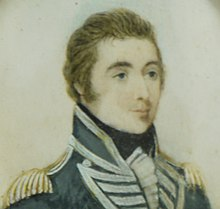
\includegraphics[height=.8\textheight]{drury}
\end{frame}

\begin{frame}
	\frametitle{Asymetrical trade and singsongs}

	\centering
	\begin{columns}
		\begin{column}{.5\textwidth}
		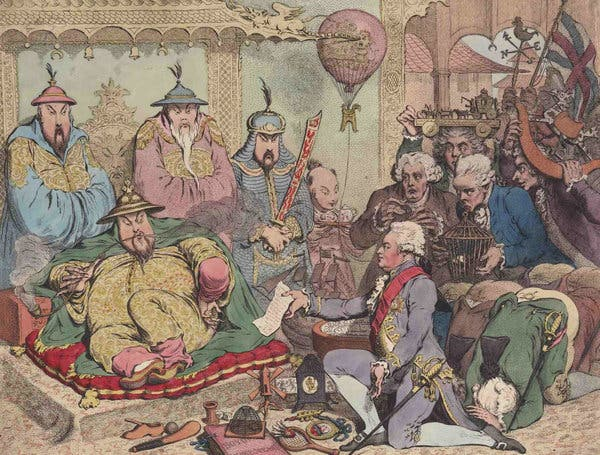
\includegraphics[width=\textwidth]{embassy}
		\end{column}
		\begin{column}{.5\textwidth}
		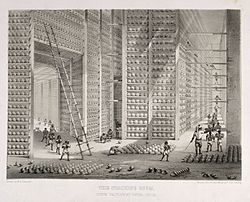
\includegraphics[width=\textwidth]{opium2}
		\end{column}

	\end{columns}
\end{frame}

\begin{frame}
	\frametitle{Language defficiences}

	
\includegraphics[width=.9\textwidth]{language}
	\note{
		Paul Norrette
	}
\end{frame}

\section{Start of war}

\begin{frame}
	\frametitle{1839 - 1860 Opium wars}
	
	\centering
	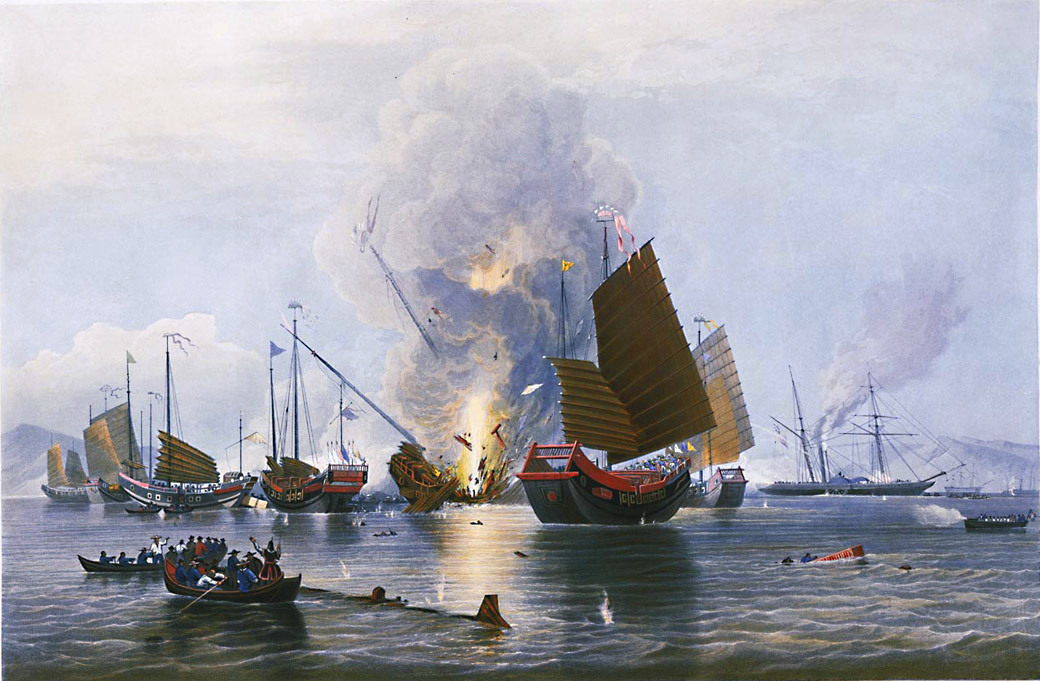
\includegraphics[height=.8\textheight]{war}
\end{frame}

\begin{frame}
	\frametitle{Outcomes of the war}

	\begin{itemize}
		\item Treaty of Nanking
		\item increased Western influence
		\item opium trade flourishes
		\item weaking the current dynasty
	\end{itemize}
\end{frame}

\end{document}
